\chapter{Implementierung}
\label{ch:implementierung}

\section{Phase 1}
Wie vorgesehen hat jedes Gruppenmitglied die Online-Platform von Rimondo genutzt um auf Bildern einer Reithalle 400 Reiter oder Pferde zu markieren. Dazu wurden Bounding Boxen um  die erkannten Reiter bzw. Pferde eingezeichnet und ein passendes Label zur Unterscheidung hinzugefügt. Die gesamten erstellten Daten wurden am Ende der Phase von Rimondo in eine Datenbank umgewandelt mit welcher in der nächsten Phase der geplante Detektor entwickelt werden sollte.

\section{Phase 2}
\subsection*{Training des Detektors}
Bevor wir mit dem Training angefangen haben, mussten wir uns in die Thematik von Image Detection sowie in die Verwendung von Mask Rcnn einlesen.

\begin{wrapfigure}{r}{0.33 \textwidth}
\scalebox{0.7}{
\begin{forest}
  pic dir tree,
  where level=0{}{% folder icons by default; override using file for file icons
    directory,
  },
  [acceptedImages
    	[img2.png, file]
 		[img3.png, file]
    	[annotations
    		[img2.csv, file]
  			[img3.csv, file]
    	]
  ]
\end{forest}
}
\caption{Ordnerstruktur Training}
\label{fig:folderstructure}
\end{wrapfigure}

Im ersten Schritt haben wir die bereitgestellten Daten aus der Datenbank aufbereitet, um diese zum Training zu verwenden. Dazu haben wir die Daten aufgeteilt, sodass pro Frame eine csv Datei mit allen Labeln und relativen Koordinaten existierte. Da jeder Frame mehrfach gelabelt wurde, haben mit einem Threshold die zusammengehörigen Dopplungen bestimmt und davon den durchschnittlichen Wert abgespeichert. 



Anschließend haben wir die hohe Auflösung der Frames verringert, um die Trainingszeit zu verkürzen. Zuletzt haben wir die Daten in einer passenden Ordnerstruktur (Abb.\ref{fig:folderstructure}) von \emph{ acceptedImages} und dem darin liegenden Ordner \emph{annotations} in ein Github Projekt eingebunden, sodass das Training von Google Colab aus erfolgen konnte.

Im zweiten Schritt haben wir die benötigten Klassen zum Training mit Mask Rcnn erstellt. Dazu wurde die Klasse RiderConfig als Unterklasse der Config Klasse erstellt, in der die Trainingsparameter individuell angepasst wurden. Wichtig war die Anzahl der zu detektierenden Klassen, die neben Reiter und Pferd auch den Hintergrund umfasst. Zudem wurde die Leistung der verfügbaren GPU sowie die Trainings- und Validierungsschritte pro Epoche angepasst.  
Weiter wurde die Klasse RiderDataset als Unterklasse der Dataset Klasse erstellt. Die nötigen Funktionen zum Laden eines Datensatzes im Trainings- und Testmodus und zum Laden der Masken, in Form  der extrahierten Boxen anhand von Eckpunkten aus den cvs Dateien, wurden darin überschrieben.

Damit konnten wir im dritten Schritt mit dem Training des Models beginnen, wozu wir ausgehend von den COCO \footnote{\href{http://cocodataset.org/}{Common Object in Context}} Gewichten Transfer Lernen verwendet haben. Für das Training haben wir unseren Datensatz in 70\% Trainings-,15 \% Test- und 15\% Validierungsdaten unterteilt. Die erste Version unseres Detektors haben wir mit 75 Epochen mit 500 Schritten trainiert. Da Mask RCNN den Loss nicht aus den Bounding Boxen, sondern auch aus den Masken berechnet, deren Genauigkeit für die Implementierung zu vernachlässigen waren, war ein Verlust unter 10 \% pro Epoche unser Zielwert. Die damit erreichte Leistung unseres Detektors war für die bereitgestellten Videos ausreichend zuverlässig (Abb. \ref{fig:SegmentierungPhase2}), sodass wir danach mit diesem die ersten Videos erstellen konnten  .

\begin{figure}
\centering
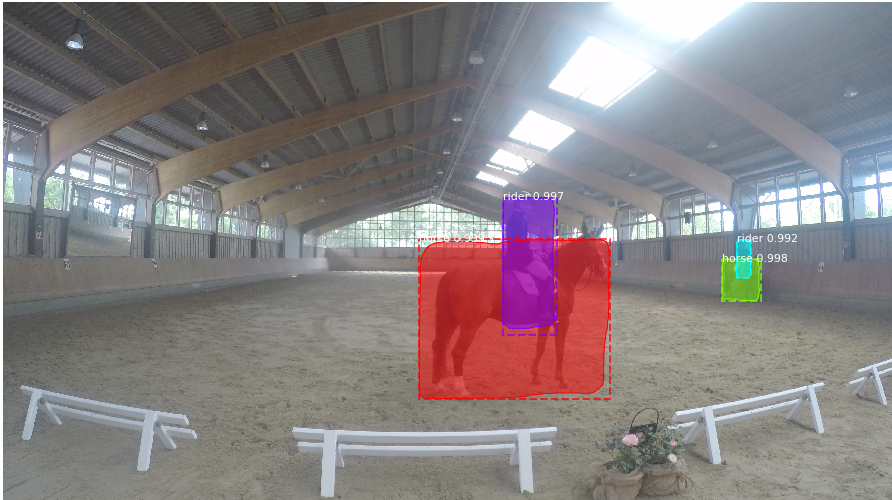
\includegraphics[height=4cm,trim={12cm 0 3cm 0},clip]{./img/IndoorMaske.png}
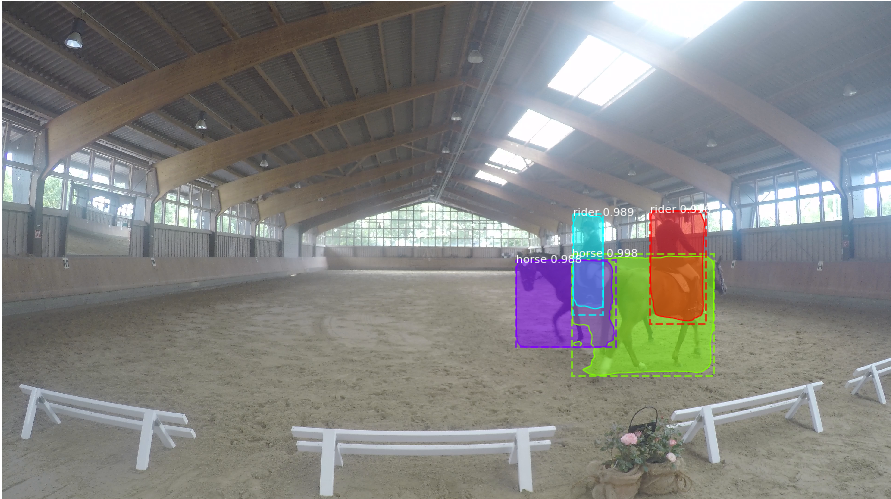
\includegraphics[height=4cm,trim={15cm 0 0 0},clip]{./img/IndoorMaske2.png}
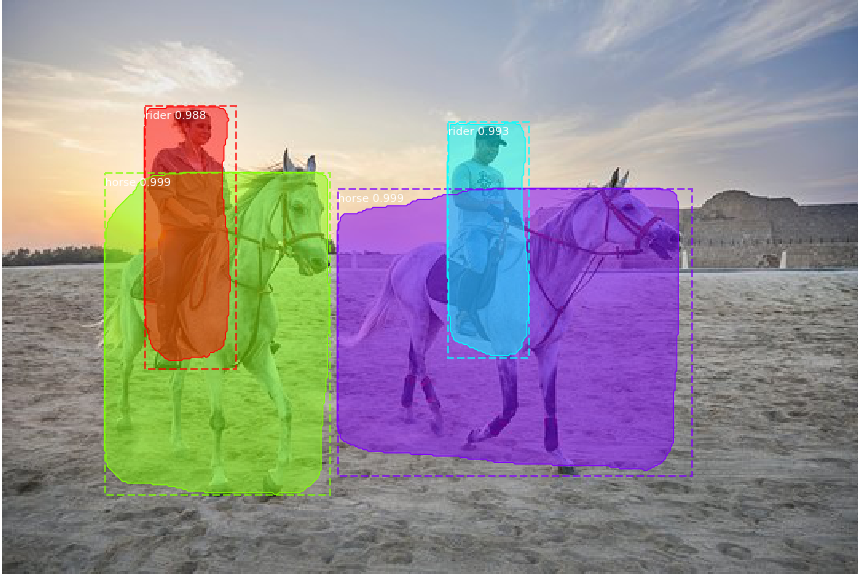
\includegraphics[height=4cm,trim={1cm 0 3cm 0},clip]{./img/OutdoorMaske.png}
\caption{Segmentierung von Reiter und Pferd nach dem Training der zweiten Phase}
\label{fig:SegmentierungPhase2}
\end{figure}

Zur vielfältigen Nutzung des erstellten Detektors, haben wir das Training mit weiteren gelabelten Bilddaten ermöglicht, um den Detektor auch in anderen Hallen zuverlässiger verwenden zu können. Dazu werden die Bilder eines Ordners nacheinander angezeigt, wobei die detektierten Pferde und Reiter mit farbigen Bounding Boxen eingezeichnet werden. Anhand dieser Boxen kann der Nutzer entscheiden, ob die Daten geeignet sind, sodass die akzeptierten Bilder und deren Boxen wie in der Ordnerstruktur von Abb.\ref{fig:folderstructure} wiederum abgespeichert werden, um den Detektor damit weiter zu trainieren.

\subsection*{Berechnung von RoIs}

Mithilfe von OpenCV werden alle Frames des Eingabevideos einzeln durchlaufen und der zuvor trainierte Detektor auf jedes einzeln angewandt. Dadurch haben wir pro Frame alle RoIs mit Bounding Boxen,als Umrandung von erkannten Reitern und Pferden, ermittelt. 

Diese Menge aus RoIs wird nun  gefiltert, da wir nur noch Reiterpaare weiter betrachten wollen. Ein Reiterpaar ist definiert als ein Mensch, der sich sehr nah an oder auf einem Pferd befindet.
Da die Bounding Boxen Rechtecke sind, können wir also berechnen, wie groß der Flächeninhalt der überlappenden Rechtecke von Reiter und Pferd ist. Ein Flächeninhalt gleich Null bedeutet dann, dass sie sich überhaupt nicht überlappen.
Dadurch ist es nicht nur möglich zu berechnen, ob ein Pferd nah an einem Menschen ist - sondern auch wie nah, indem wir einen Threshold gewählt haben, der die Größe des errechneten Flächeninhalts prüft. Beispielsweise hätte ein Mensch \emph{auf} einem Pferd einen größeren Flächeninhalt als ein Mensch \emph{neben} einem Pferd, was je nach Wunsch also angepasst werden kann.
Wenn eine Mensch-RoI also eine Pferd-RoI überlappt, zeichnen wir um beide eine Reiterpaar-RoI. Damit haben wir einzelne Pferde, Reiter und Fehldetektionen vom Tracking ausgeschlossen.

Wir verfolgten hier den Ansatz zunächst alle Reiterpaare in den RoIs abzubilden und uns erst in der dritten Phase selektiv auf ein einzelnes Paar zu fokussieren. Dieser Modus kann weiterhin gut für Aufwärmphasen der Reitturniere genutzt werden, bei denen mehrere Reiterpaare auf dem Turnierplatz sind. Die Umsetzung ist als austauschbarer Filter konzipiert, der eine Gesamtbox anhand der maximalen und minimalen Eckpunkte aller detektierten Bounding Boxen bestimmt.
Ausgehend von der Gesamtbox müssen für die Erstellung erster Videos noch nötige Sonderfälle beachtet werden. So wird der Zoom unter 240 Pixel verhindert, um eine gute Bildqualität zu ermöglichen. Die längere Seite der Bounding Box ist ausschlaggebend für die Berechnung der passenden Ratio des Bildausschnittes, sodass dann die optimalen  Eckpunkte berechnet werden können. Wichtig ist es noch die Ränder des Sichtfeldes zu berücksichtigen und die Ratio entsprechend zu korrigieren.
Im letzten Schritt werden die Rois mithilfe der kalkulierten Gesamtbox aus jedem Frame ausgeschnitten und auf die selbe Größe skaliert, was durch die gleiche Ratio aller Frames keine Verzerrung zur Folge hat, und ein Ausgabevideo geschrieben.





\section{Phase 3}
\subsection*{Weiterentwicklung des Detektors}

\begin{figure}
\centering
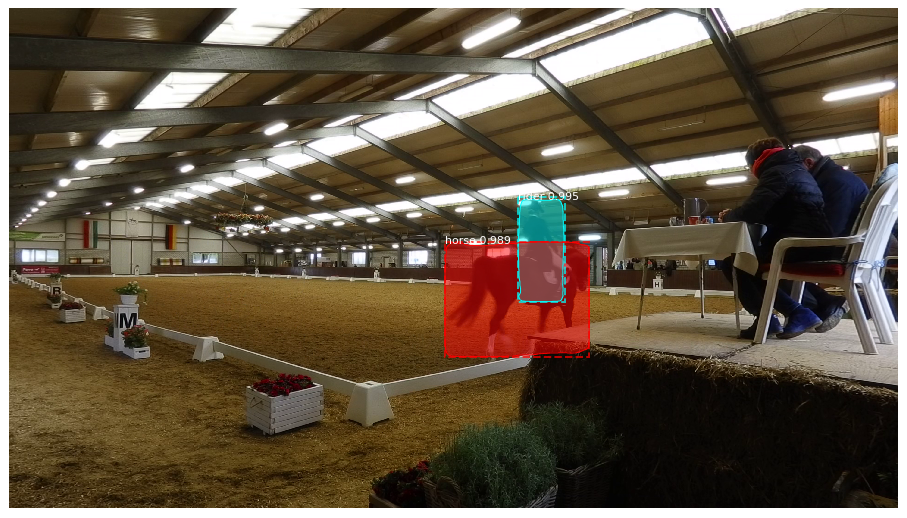
\includegraphics[height=4cm,trim={6cm 0 6cm 0},clip]{./img/IndoorMask6.png}
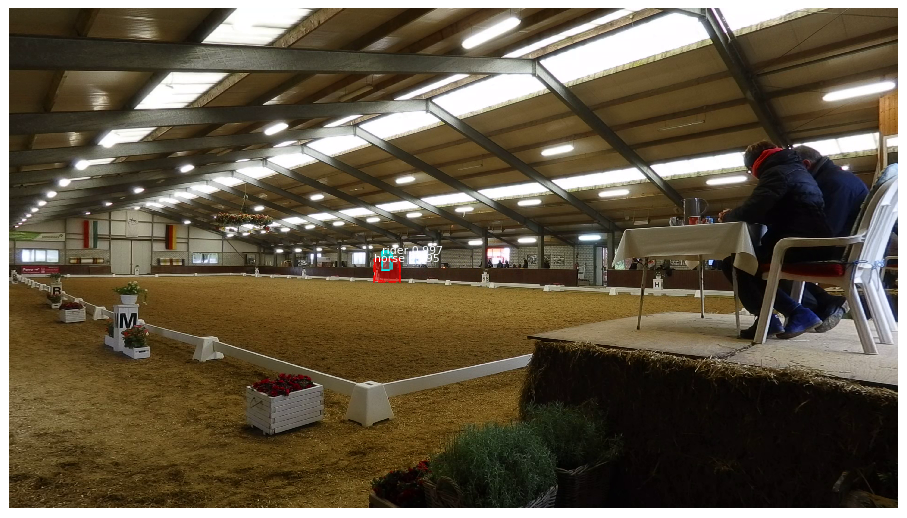
\includegraphics[height=4cm,trim={6cm 0 6cm 0},clip]{./img/IndoorMask3.png}
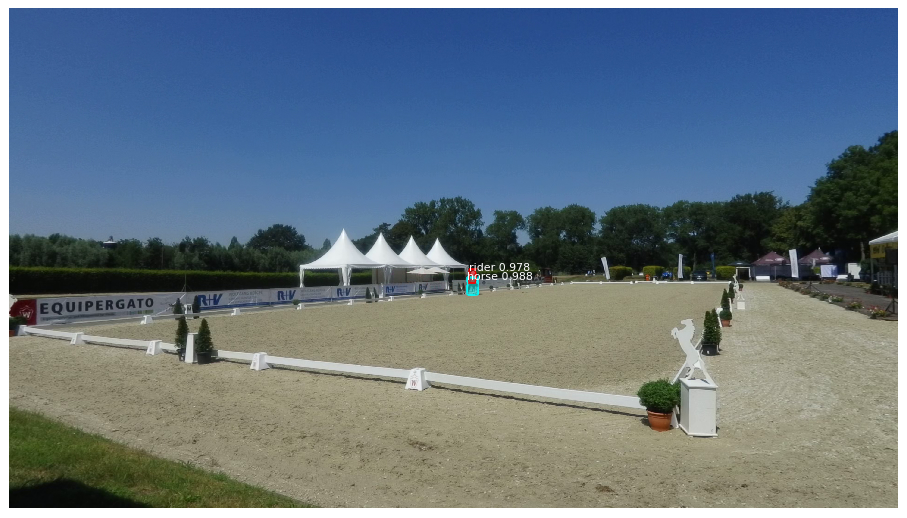
\includegraphics[height=4cm,trim={6cm 0 6cm 0},clip]{./img/OutdoorMask2.png}
\caption{Segmentierung von Reiter und Pferd nach dem Training der zweiten Phase}
\label{fig:SegmentierungPhase3}
\end{figure}

Mit Beginn der dritten Phase wurden weitere Reitvideos zur Verfügung gestellt, welche in verschiedenen Hallen sowie im Außenbereich gefilmt wurden. Der erste Test mit dem Detektor der zweiten Phase verlief nicht sonderlich zufriedenstellend, wodurch wir mehrere Probleme identifizieren konnten. Zum einen wurden nicht alle Reiter und Pferde, die weit entfernt von der Kamera waren, korrekt detektiert. Dieses Ergebnis war aufgrund des zuvor recht einseitigen Trainings nicht verwunderlich, da sich die Hintergründe, Reiter und Pferde unterschieden. Zum anderen wurden auch viele sitzende Personen als Reiter identifiziert und einige Gegenstände wie beispielsweise Pflanzen als fehlerhaft erkannt. Nachdem wir jedoch ungefähr 500 weitere Frames pro neuer Umgebung ausgewählt und damit den Detektor weiter trainiert hatten, wurden ein Großteil der Fehler beseitigt (Abb. \ref{fig:SegmentierungPhase3}). Durch die Erweiterung des Detektors ist dieser nun auch in der Lage unterschiedlich gekleidete Reiter und Pferde mit abweichende Fellfarben zuverlässiger zu detektieren.


\subsection*{Benutzeroberfläche}

\begin{figure}[b]
\centering
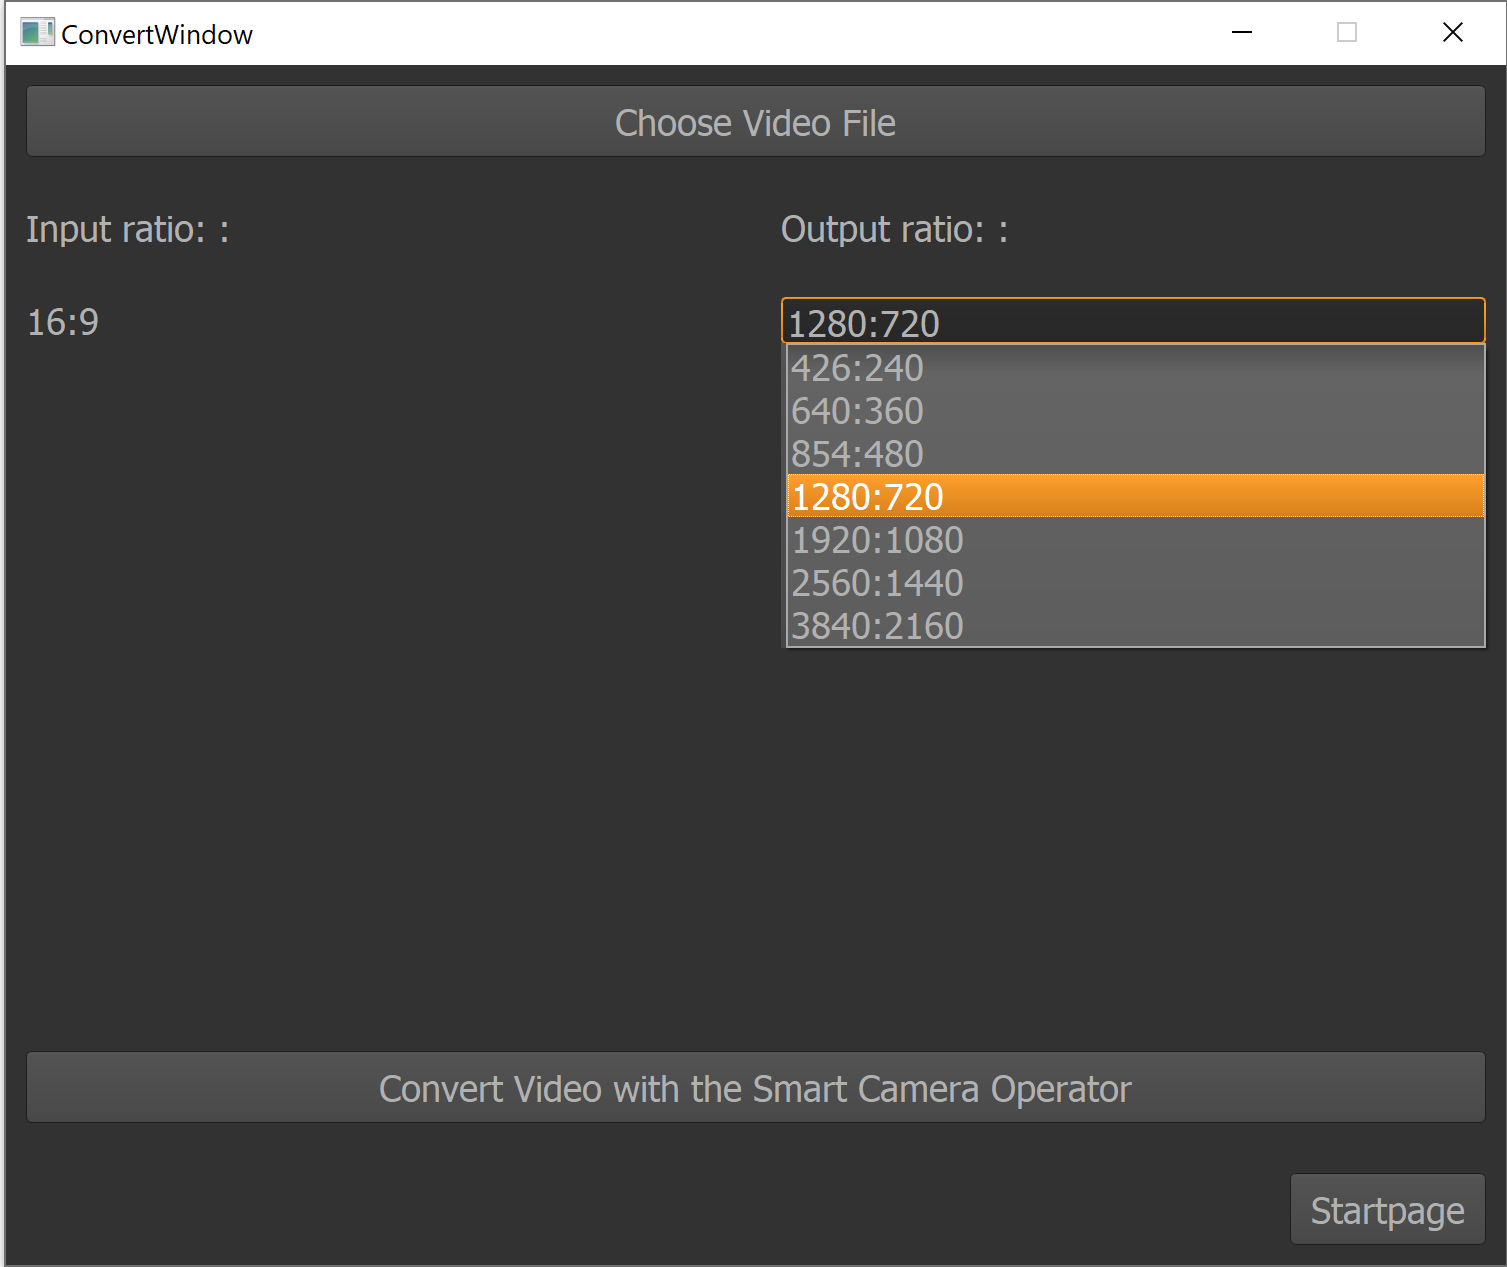
\includegraphics[width=0.45\textwidth]{./img/GuiConvert2.png}
%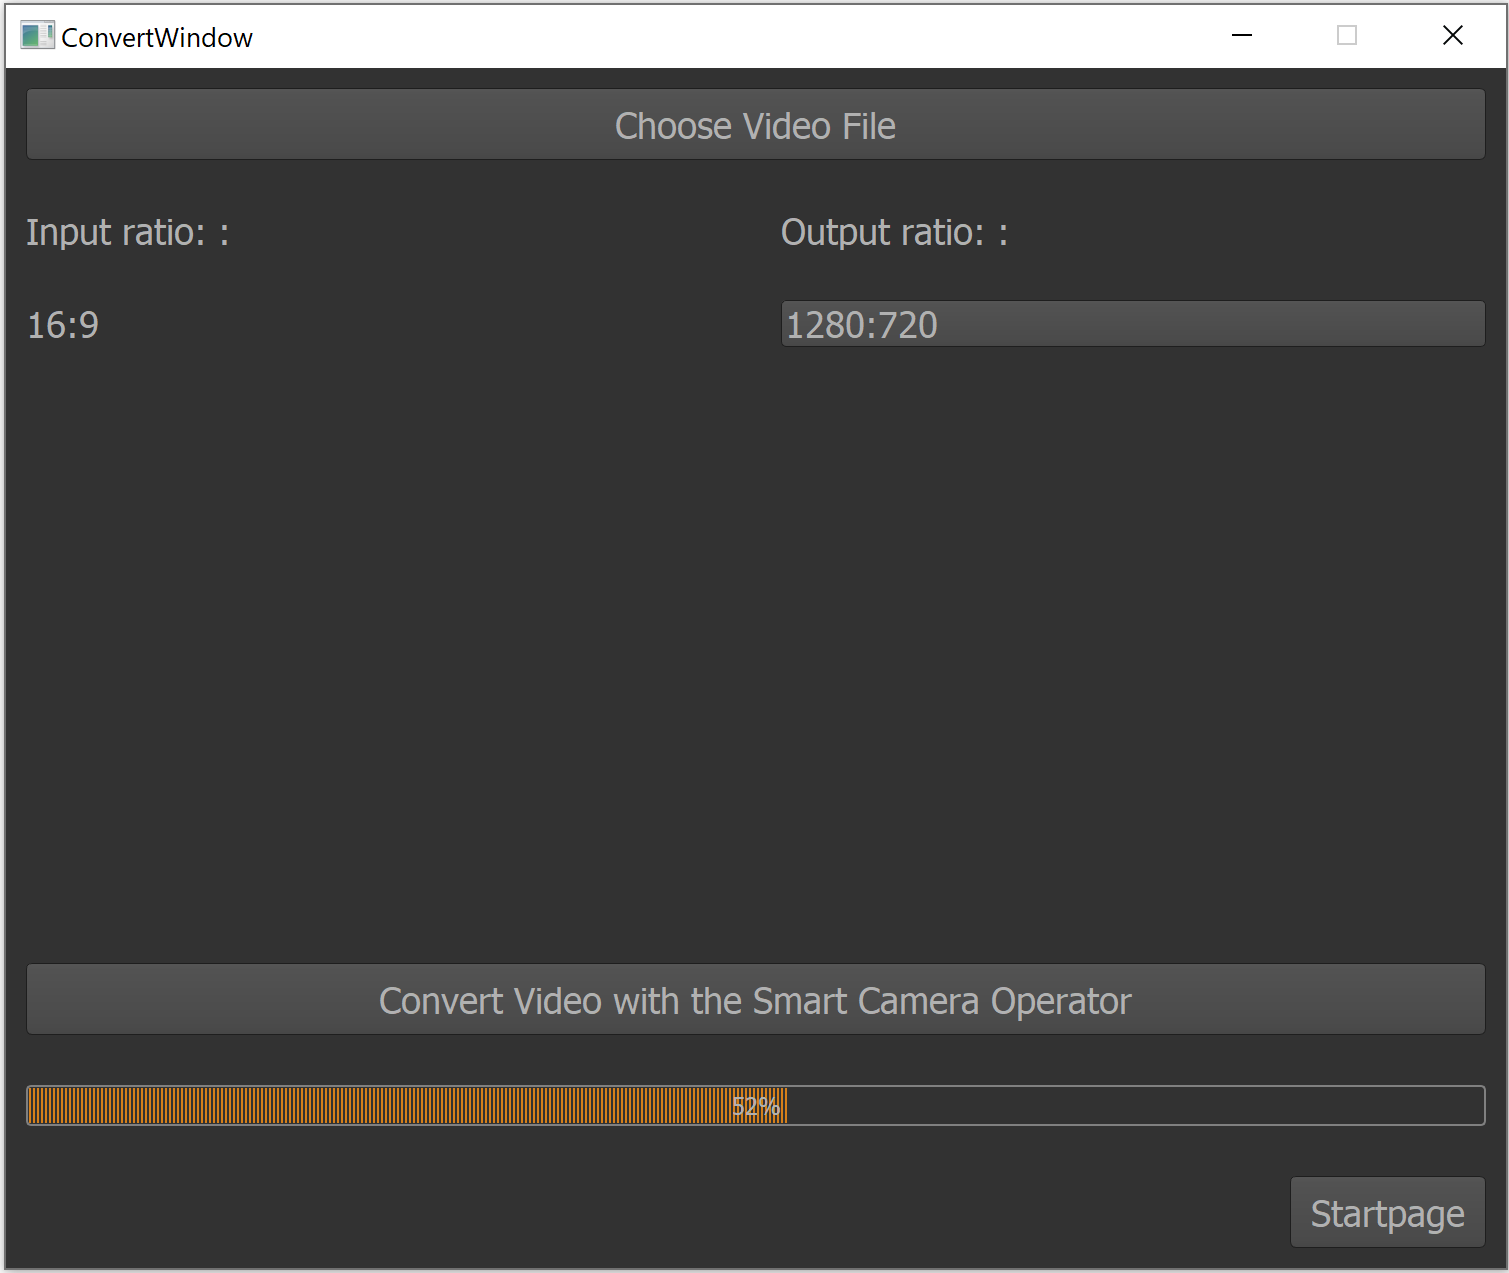
\includegraphics[width=0.32\textwidth]{./img/GuiConvert.png}
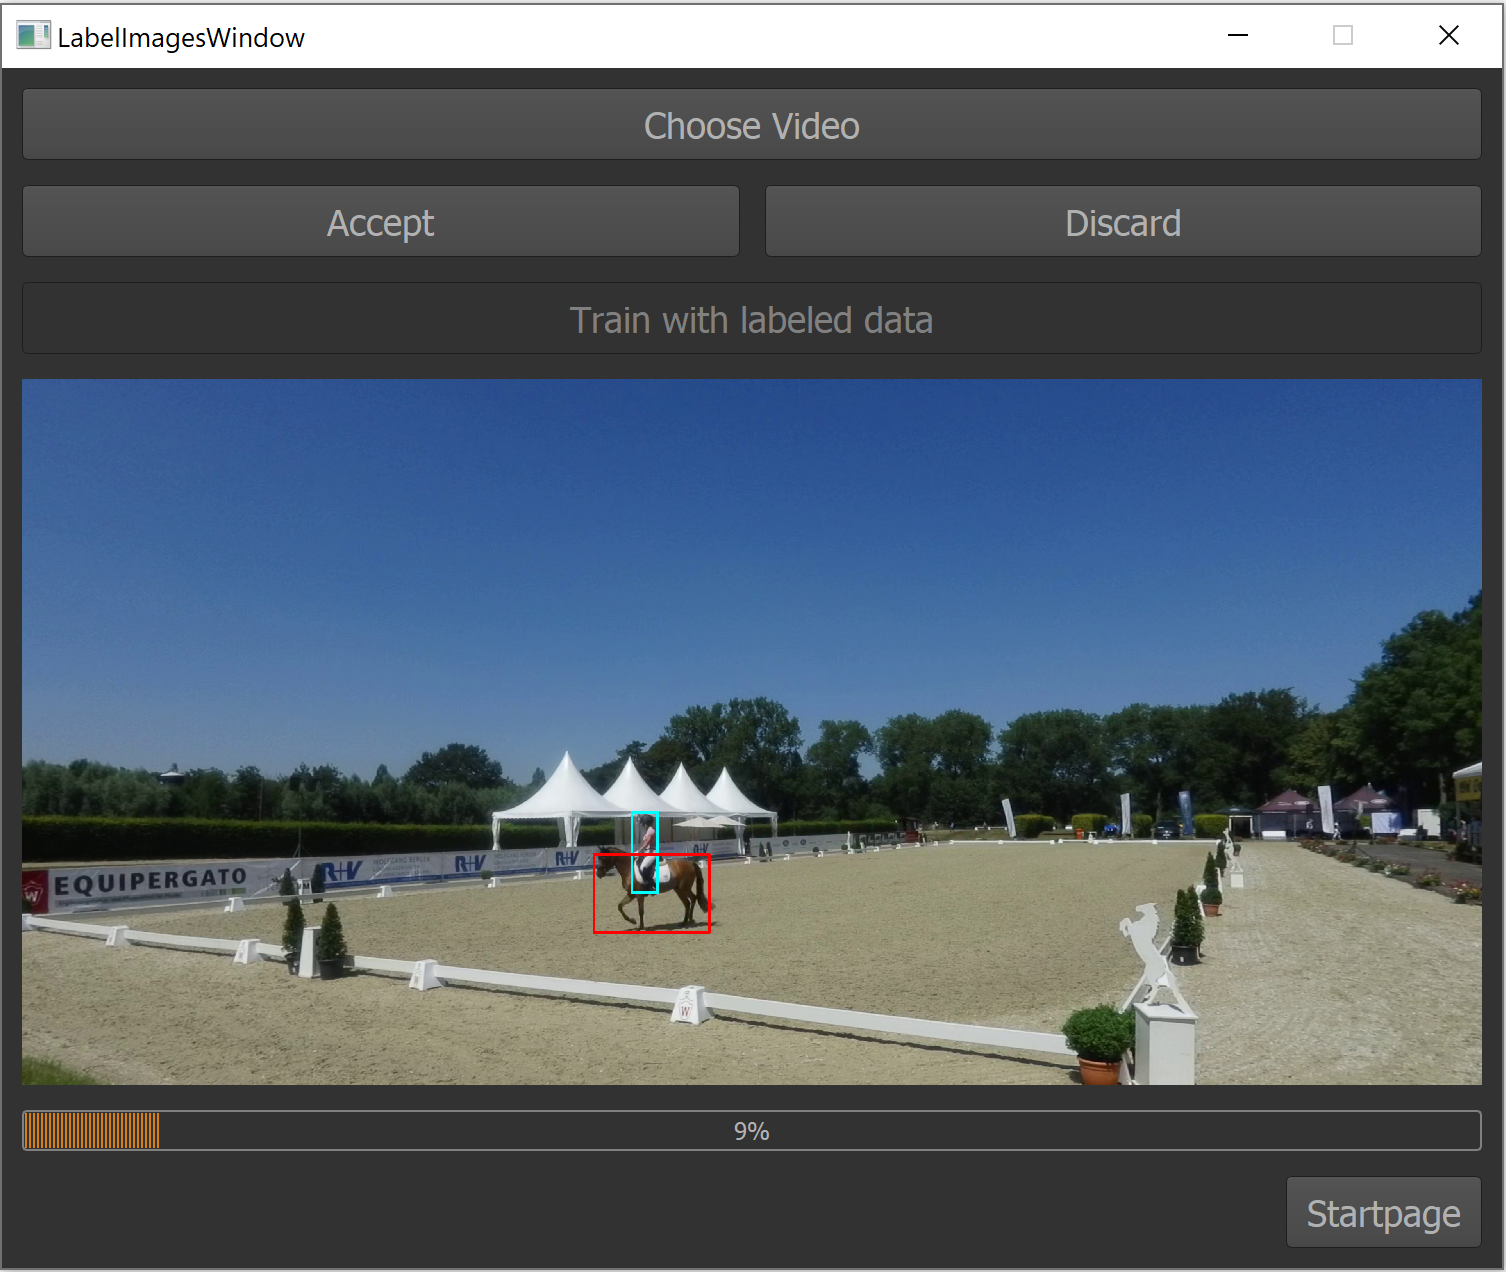
\includegraphics[width=0.45\textwidth]{./img/GuiLabel.png}
\caption{Benutzeroberläche Konvertieren und Labeln eines Videos}
\label{fig:gui}
\end{figure}

Im Hinblick auf die Kundengruppe haben wir das Kennzeichnung weiterer Bilddaten und die Konvertierung eines Videos für autonome Kameraführung in eine GUI eingebunden. Die GUI wurde mit PyQt5 erstellt und das Standardaussehen durch Einbinden eines Stylesheets modifiziert. Mit dieser minimalen Benutzeroberfläche kann der Nutzer nun zunächst auswählen ob weitere Daten gelabelt oder ein Video umgewandelt werden soll (Abb.\ref{fig:gui}). Bei der Auswahl weiterer Bilddaten können sowohl Ordner mit Bildern als auch Videos mithilfe extrahierter Frames verwendet werden. Dazu kann der Nutzer pro Bild entscheiden ob die eingezeichnete Detektion akzeptiert oder abgelehnt wird und den Detektor im Anschluss damit weiter trainieren. Für die Umwandlung eines Videos wird nach Auswahl der Datei und der Auflösung des Ausgabeformates ein Video mithilfe des Smart Camera Operators erstellt.


\subsection*{Performance}
Da der Fokus unserer Gruppe auf der Genauigkeit des Detektors liegt, haben wir nur einige grundlegende Verbesserungen der Performance vorgenommen, welche dem nicht entgegenwirken. 
Im ersten Schritt wird dazu anhand der Auflösung des Eingabevideos entschieden, ob die Frames vor der Detektion verkleinert werden sollten. Dies war bei den aufgenommenen Videos mit 4K Auflösung sinnvolle, da Mask Rcnn auch mit einfacher HD Auflösungen ähnlich gute Ergebnisse liefert. Somit konnte der Zeitaufwand der Detektion von ca. 0.81  auf ca. 0.48 Sekunden pro Detektion verbessert werden. Anschließend müssen die detektierten Boxen wieder entsprechend hochskaliert werden, um mit den Ursprungsbilder übereinzustimmen.

Zur weitere Verbesserung haben wir den Einsatz von Ausgleichsgeraden und Ausgleichskurven getestet. Als Ansatz haben wir den Gedankengang verfolgt, nicht für jeden Frame Detektionen durchzuführen, sonder nur für jeden \linebreak n-ten Frame, wodurch die Anwendung beschleunigt würde. 
In beiden Fällen haben wir mithilfe von Numpy die Berechnungen mit \emph{polyfit} anhand der letzten 10 Detektionen erstellt. Die Ergebnisse für die Ausgleichsgerade stellten sich zwar performancemäßig als sehr positiv dar, jedoch nahm die Videoqualität stark ab. Das Ausgabevideo wies aufgrund der Ausgleichsgeraden sehr regelmäßige gerade Kameratranslationen auf, die die Gesamtqualität verminderten.
Als nächstes nutzten wir statt der Geraden Ausgleichskurven, wobei sich bereits Kurven vom Grad 2 oder 3 ausreichend gut eigneten. Während dadurch die vorherigen Makel im Ausgabevideo gelöst wurden, stellte sich nur sehr geringfügiger bis gar kein Performacevorteil heraus. Aufgrund dessen wurden beide Versuche die Anzahl der Detektionen zu verringern verworfen und aus Zeitgründen nicht weiter verfolgt.




\subsection*{Videoqualität}
Der Schwerpunkt der Phase richtet sich auf ein robusteres und flüssigeres Tracking, was wir mit besonderen Fokus auf Ausnahmesituationen und die Qualität der Kameraführung umgesetzt haben.



\subsubsection*{Tracking}
Da der Detektor nicht komplett fehlerlos ist und demnach ein uninteressantes und entferntes Objekt für einen Zeitraum auch mal priorisieren kann, ist es wichtig diese Sprünge zu unterbinden. Ein Reiterpaar bewegt sich im Normalfall nicht innerhalb 2 Frames über den ganzen Platz, der Abstand des Reiterpaares zu seiner Position auf dem vorherigen Bild ist also relativ gering. Um diese Sprünge zu vermeiden prüfen wir also, ob die Position des getrackten Objektes des aktuellen Bildes stark von der Position des vorherigen getrackten Objektes abweicht. Damit der Wert der vorherigen Position als relativ akkurat gelten kann, nehmen wir, statt nur die Position des vorletzen Bildes, den Median der letzten 25 getrackten Boxen. Sollte nun die Distanz einen Schwellwert überschreiten, wird die neue Box ignoriert und für das aktuelle Bild die zuletzt valide Box verwendet. Damit der Smart Camera Operator nicht auf einer Position hängen bleibt, ist ein Sicherungsmechanismus eingebaut, der ihn wieder zurücksetzt und neues Tracking erlaubt.

Sollte das Reiterpaar sich hinter einem Hindernis verstecken oder aus dem Bild hinauslaufen, wird die Kamera an der zuletzt gesichteten Stelle verbleiben bis das Paar wieder sichtbar geworden ist oder ein neues Paar detektiert wird.

\subsubsection*{Glättung}
Um die Folge der RoIs zu glätten, damit sich nach dem Zuschneiden ein sanftes Seherlebnis für den Zuschauer bietet, haben wir verschiedene Verfahren ausprobiert.
Das effektivste, effizienteste und gleichzeitig das einfachste Verfahren, das zum Einsatz kam, war ein eindimensionaler Gaußfilter.
Wir haben eine Folge aus RoIs, dabei hat jedes RoI 4 Attribute - die Koordinaten $(x1,y1), (x2,y2)$ der linken unteren und rechten oberen Ecke des Rechtecks.
Wir verwenden für alle Koordinaten $x1, y1, x2, y2$ aller RoIs einen  eindimensionalen Gaußfilter mit $\sigma=5$, genauer nutzen wir also insgesamt vier Mal einen Filter über die RoIs für jede der vier Koordinaten.

Eine weitere Möglichkeit wäre es gewesen, die Richtungsänderungen zu erkennen oder zu berechnen und dann einfach die RoIs linear von einer Richtungsänderung zur nächsten wandern zu lassen, was sich beispielsweise mit \emph{optical flow} berechnen lässt. Das wäre auch für die Echtzeit-Anwendung nötig gewesen, bei der die Kamerabewegung and der Position des getrackten Objektes orientieren soll.
Da wir aber für unseren Anwendungsfall einen effizientere Möglichkeit gefunden haben und Live-Übertragungen den Umfang des Praktikums überschreiten, haben wir dies nicht weiter thematisiert und implementiert. 
